\documentclass[11pt, a4]{article}
\usepackage{qtree}
\usepackage{amsmath}
\usepackage{amssymb}
\usepackage{mathtools}
\usepackage{tikz}

\usetikzlibrary{positioning}
\newcommand\tab[1][0.5cm]{\hspace*{#1}}

%% define left/right/full outer join symbols
\def\ojoin{\setbox0=\hbox{$\bowtie$}%
  \rule[-.02ex]{.25em}{.4pt}\llap{\rule[\ht0]{.25em}{.4pt}}}
\def\leftouterjoin{\mathbin{\ojoin\mkern-5.8mu\bowtie}}
\def\rightouterjoin{\mathbin{\bowtie\mkern-5.8mu\ojoin}}
\def\fullouterjoin{\mathbin{\ojoin\mkern-5.8mu\bowtie\mkern-5.8mu\ojoin}}
\newcommand*{\QEDB}{\null\nobreak\hfill\ensuremath{\square}}%

\setcounter{section}{1}
\begin{document}
\title{Exercise Sheet 3}

\section*{Exercise Sheet 3}
\subsection*{Exercise 1}
Give the query graphs for the two queries from the first exercise sheet.
\begin{verbatim}
SELECT s1.name
FROM studenten s1
JOIN hoeren h1 ON s1.matrnr = h1.matrnr
JOIN hoeren h2 ON h1.vorlnr = h2.vorlnr
JOIN studenten s2 ON h2.matrnr = s2.matrnr
WHERE s2.name = 'Schopenhauer'
AND s1.name != 'Schopenhauer';
\end{verbatim}
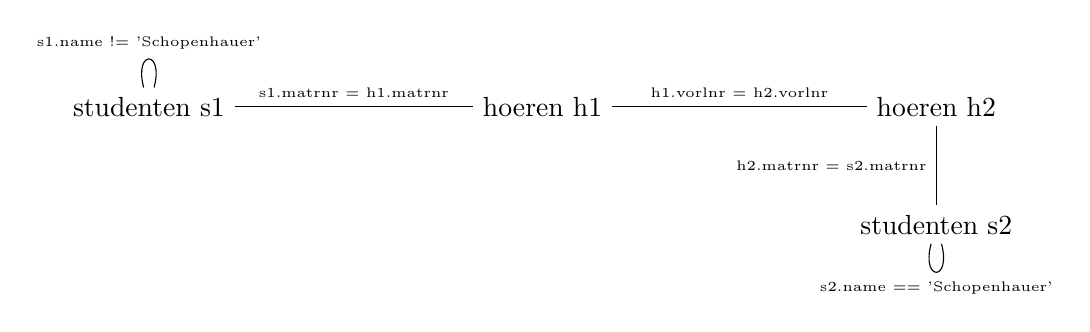
\begin{tikzpicture}[node distance=5cm]
  \tikzset{every loop/.style={}}%removes arrow head from all loops.
  \node (s1) at (0,0) {studenten s1};
  \node (h1) [right of=s1] {hoeren h1};
  \node (h2) [right of=h1] {hoeren h2};
  \node (s2) [below=1cm of h2] {studenten s2};
  \draw (s1) -- (h1) node[pos=0.5,above] {\tiny s1.matrnr = h1.matrnr};
  \draw (h1) -- (h2) node[pos=0.5,above] {\tiny h1.vorlnr = h2.vorlnr};
  \draw (h2) -- (s2) node[pos=0.5,left] {\tiny h2.matrnr = s2.matrnr};
  \draw (s1) edge [loop above] node {\tiny s1.name != 'Schopenhauer'} (s1);
  \draw (s2) edge [loop below] node {\tiny s2.name == 'Schopenhauer'} (s2);
\end{tikzpicture}


\begin{verbatim}
SELECT p.persnr, p.name
FROM professoren p
JOIN vorlesungen v ON v.gelesenvon = p.persnr
JOIN hoeren h1 ON h1.vorlnr = v.vorlnr
JOIN hoeren h2 ON h2.vorlnr = h1.vorlnr
WHERE h1.matrnr != h2.matrnr;
\end{verbatim}
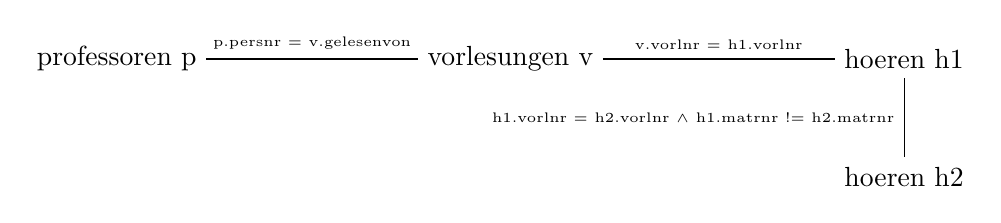
\begin{tikzpicture}[node distance=5cm]
  \node (p) at (0,0) {professoren p};
  \node (v) [right of=p] {vorlesungen v};
  \node (h1) [right of=v] {hoeren h1};
  \node (h2) [below=1cm of h1] {hoeren h2};
  \draw (p) -- (v) node[pos=0.5,above] {\tiny p.persnr = v.gelesenvon};
  \draw (v) -- (h1) node[pos=0.5,above] {\tiny v.vorlnr = h1.vorlnr};
  \draw (h1) -- (h2) node[pos=0.5,left] {\tiny h1.vorlnr = h2.vorlnr $\land$ h1.matrnr != h2.matrnr};
\end{tikzpicture}

\newpage
\subsection*{Exercise 2}
$|R_1| = 1, |R_2| = 40, |R_3| = 40, |R_4| = 1, f_{1,2} = 0.75, f_{2,3} = 0.01, f_{3,4} = 0.75$\\
\vspace{.2cm}\\
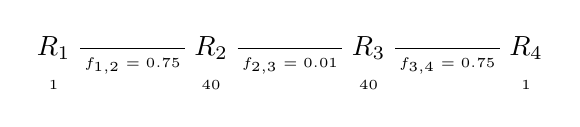
\begin{tikzpicture}[node distance=2cm]
  \node (R1) at (0,0) {$R_1$};
  \node (R2) [right of=R1] {$R_2$};
  \node (R3) [right of=R2] {$R_3$};
  \node (R4) [right of=R3] {$R_4$};
  \draw (R1) -- (R2) node[pos=0.5,below] {\tiny $f_{1,2} = 0.75$};
  \draw (R2) -- (R3) node[pos=0.5,below] {\tiny $f_{2,3} = 0.01$};
  \draw (R3) -- (R4) node[pos=0.5,below] {\tiny $f_{3,4} = 0.75$};
  \node (CR1) [below=0.01cm of R1] {\tiny{1}};
  \node (CR2) [below=0.01cm of R2] {\tiny{40}};
  \node (CR3) [below=0.01cm of R3] {\tiny{40}};
  \node (CR4) [below=0.01cm of R4] {\tiny{1}};
\end{tikzpicture}\\
\vspace{.2cm}\\
\begin{tabular}{l|r|r}
    $X$ & $C_{\text{out}}$ & $|X|$\\
    \hline
    $R_1 \bowtie R_2$ & 30 & 30\\
    $R_2 \bowtie R_3$ & 16 & 16\\
    $R_3 \bowtie R_4$ & 30 & 30\\
    &&\\
    $R_1 X R_3$ & 40 & 40\\
    $R_1 X R_4$ & 1 & 1\\
    \hline
    $(R_1 \bowtie R_2)\bowtie R_3$ & 42 & 12\\
    $(R_2\bowtie R_3) \bowtie R_1$ & 28 & 12\\
    &&\\
    $(R_1 X R_3)\bowtie R_2$ & 52 & 12\\
    $(R_1 X R_3)\bowtie R_4$ & 70 & 30\\
    $(R_1 X R_4)\bowtie R_2$ & 31 & 30\\
    \hline
    $(R_1 \bowtie R_2)\bowtie (R_3 \bowtie R_4)$ & 69 & 9\\
    $(R_1 X R_3)\bowtie (R_2 X R_4)$ & 90 & 9\\
    \textcolor{red}{$(R_1 X R_4)\bowtie (R_2 \bowtie R_3)$} & \textcolor{red}{26} & \textcolor{red}{9}\\
    &&\\
    $((R_1 \bowtie R_2)\bowtie R_3) \bowtie R_4$ & 51 & 9\\
    $((R_2 \bowtie R_3)\bowtie R_1) \bowtie R_4$ & 37 & 9\\
    $((R_1 X R_3)\bowtie R_2) \bowtie R_4$ & 61 & 9\\
    $((R_1 X R_3)\bowtie R_4) \bowtie R_2$ & 79 & 9\\
    $((R_1 X R_4)\bowtie R_2) \bowtie R_3$ & 40 & 9\\
\end{tabular}

\end{document}
